\documentclass{article}

% \usepackage{standalone}
 \usepackage{graphicx}
% \usepackage{media9}
%\graphicspath{{./images/}}
% \usepackage{amsmath}
% \usepackage{setspace}                       \usepackage{geometry}          
%  \usepackage{longtable}                      
% \usepackage{chicago}                  
% \usepackage{times} 
% \usepackage{paracol}   % parallel columns    
% \usepackage[dvipsnames]{xcolor}       \usepackage{calc}                                      

% \usepackage{tikz}
% \usetikzlibrary{positioning, shadows, arrows, automata, shapes, calc, decorations.pathreplacing,calligraphy}
\begin{document}


\section{Change wealth sensitivity 12-15 -010050}
no sensitivity

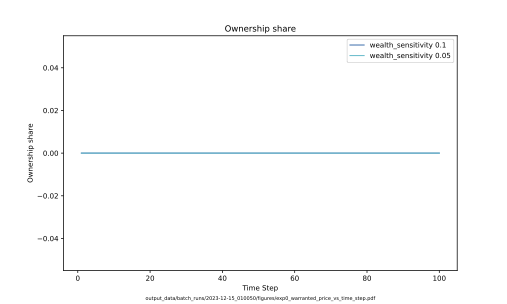
\includegraphics[scale=.45]{fig/Analysis/exp0_warranted_price_vs_time_step.png}

\subsection{parameters}
\begin{verbatim}

  'adjn': 0.15,
            'adjF': 0.02,
            'adjw': 0.05, 

 'capital_gains_tax_person':   0.0, # share 0-1

'capital_gains_tax_investor': 1, # share 0-1 
\end{verbatim}
---
\newpage
\section{Change adjF - the growth rate of number of firms }
\begin{tabular}{c|c}
  mpl   &  up\\
  n   &  dn\\
  N   &  up\\
  F   & up \\
  E   &  up\\
  k   & dn
\end{tabular} 

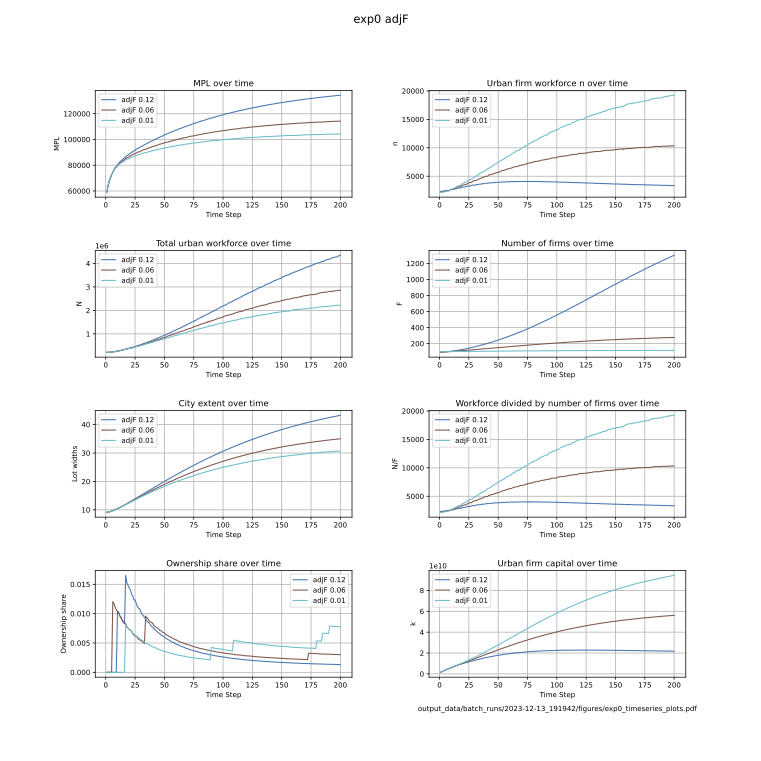
\includegraphics[scale=.75]{fig/Analysis/2023-12-13-91942-timeseries-plots.png}

\newpage
% \subsection{parameters}
% \begin{verbatim}

% \end{verbatim}


% \section{Change  12-15 010050}
\begin{tabular}{c|c}
  mpl  &  \\
  n   &  \\
  N   &  \\
  F   &  \\
  E   &  \\
  k   & 
\end{tabular} 

% \includegraphics[scale=.25]{}


% \subsection{parameters}
% \begin{verbatim}

% \end{verbatim}
\newpage
% \subsection{parameters}
% \begin{verbatim}

% \end{verbatim}


% \section{Change  12-15 010050}
\begin{tabular}{c|c}
  mpl  &  \\
  n   &  \\
  N   &  \\
  F   &  \\
  E   &  \\
  k   & 
\end{tabular} 

% \includegraphics[scale=.25]{}

 \end{document}

 \newpage
% \subsection{parameters}
% \begin{verbatim}

% \end{verbatim}

% \section{Change  12-15 010050}
\begin{tabular}{c|c}
  mpl  &  \\
  n   &  \\
  N   &  \\
  F   &  \\
  E   &  \\
  k   & 
\end{tabular} 

% \includegraphics[scale=.25]{}
